\documentclass{article}
\usepackage{lipsum}
% Language setting
% Replace `english' with e.g. `spanish' to change the document language
\usepackage[english]{babel}
% Set page size and margins
% Replace `letterpaper' with `a4paper' for UK/EU standard size
\usepackage[letterpaper,top=2cm,bottom=2cm,left=3cm,right=3cm,marginparwidth=1.75cm]{geometry}

% Useful packages
\usepackage{amsmath}
\usepackage{graphicx}
\usepackage{subcaption}
\usepackage{wrapfig}
\usepackage{pdfpages}
\usepackage{lipsum}
% \usepackage[colorlinks=true, allcolors=blue]{hyperref}

\usepackage{color}   %May be necessary if you want to color links
\usepackage{hyperref}
\hypersetup{
    colorlinks=true, %set true if you want colored links
    linktoc=all, 
    linkcolor=blue,
}
\usepackage{cleveref}
% More defined colors
\usepackage[dvipsnames]{xcolor}

% Required package
\usepackage{tikz}
\usetikzlibrary{positioning}

\title{Foundations of Deep Learning}
\author{Geralyn Chong}
\begin{document}
\maketitle
\tableofcontents

\vspace{10pt}
\begin{small}
Note: This is a brief set of notes that I took during the day. Feel free to add to the latex and update me so I can update the master doc!
\end{small}

\section{Useful Links:}
\begin{enumerate}
    \item \href{https://catalog.ngc.nvidia.com/orgs/nvidia/containers/dli-dl-fundamentals}{Nvidia Container to running Fundamentals of Deep Learning}
    \item PDFs of the Workshop's Slides:
    \begin{itemize}
        \item \href{https://drive.google.com/file/d/1IJbwErD_sPRxy15AlihhnK6s7yEMlci_/view?usp=drive_link}{Slide 1}
        \item \href{https://drive.google.com/file/d/1wIJISrSTmXjoDfUpvk4yGvzBWxXGaXKL/view?usp=sharing}{Slide 2}
        \item \href{https://drive.google.com/file/d/1tT1qHztY3PxpvqJ6jeBhF67t4TYbMtiD/view?usp=drive_link}{Slide 3}
        \item \href{https://drive.google.com/file/d/1v2rKuM5UdxolFZd2iy8b36yGFi_0bmur/view?usp=sharing}{Slide 4}
        \item \href{https://drive.google.com/file/d/1HoWBOPXJSpdl1rIhvSN0EBnoO0VdJYEh/view?usp=drive_link}{Slide 5}
        \item \href{https://drive.google.com/file/d/1aK88wA-z32ZiDT_4isxbjv6FK_aXuM_V/view?usp=drive_link}{Slide 6}
    \end{itemize}
\end{enumerate}
\section{History of AI}
\subsection{Early Neural Networks}
\begin{itemize}
    \item Inspired by biology $\rightarrow$ Von Neumann Architecture
    \item \textbf{Expert Systems} aids the "intelligence" of old computer systems; Built to mimic a human expert; 
    \begin{itemize}
        \item But we don't want to hard code these complex conditions of real world problems! 
        \item Training models like training children to recognize important relationships and patterns on their own by exposing them to data etc. 
    \end{itemize}
\end{itemize}
\subsection{The Deep Learning Revolution}
\begin{enumerate}
    \item \textbf{Data}
        Networks need a lot of data via the internet
    \item \textbf{Processing Power}
    \item \textbf{Importance of the GPU}
        Matrix multiplication applies to graphic rendering (animation, simulation, etc.) Parallel processing - help to execute these operations millions of times. 
\end{enumerate}

\section{What is Deep Learning?}
\subsection{Traditional Programming}
\begin{enumerate}
    \item Define a set of rules for classification
    \item Program those rules into a computer
    \item Feeback
\end{enumerate}
\subsection{Deep Learning steps...}
If the rules are nuanced, complex, use deep learning. Taking in real world conditions that are hard to describe. 
\begin{enumerate}
    \item Show modle the examples with the answer of how to classify
    \item Takes guesses
    \item Model learns to correctly cateogirze as its training. System \textbf{LEARNS} these rules on their own
\end{enumerate}
Deep Learning has a large depth ond complexity of layers and networks. 
\section{Hello Neural Networks}
\begin{itemize}
    \item Train a network to correctly classify handwritten digits
    \item Try learning like a neural network
    \item \href{https://build.nvidia.com/}{Cool sandbox link}
\end{itemize}

\section{\href{http://dli-e5d62e622240-a8611b.westus3.cloudapp.azure.com/lab/lab/tree/01_mnist.ipynb}{Lab 1: Mnist Dataset}}
\subsection{Validation vs Test}
\begin{enumerate}
    \item Validation and Test sets are held out from the training process because evaluating models based on the same data that we train them on would result in bias
    \item Training set refers to a set of examples that we want to pass through the model in order to learn specific rules. However, we can use the verification set to \textit{fine-tune} the model (e.g choosing the number of hidden units in a neural network). Test set used to evaluate the performance of the model. Pseudocode: 
    \begin{verbatim}
# split data
data = ...
train, validation, test = split(data)

# tune model hyperparameters
parameters = ...
for params in parameters:
	model = fit(train, params)
	skill = evaluate(model, validation)

# evaluate final model for comparison with other models
model = fit(train)
skill = evaluate(model, test)
    \end{verbatim}
\end{enumerate}
\subsection{However, just a validation set is not enough!}
Another method that can be used is the \textbf{k-fold cross validation method}. This method aims to mitigate against biases when dividing large datasets randomly. With smaller datasets, we might be overfitting towards a specific division of points and failing the test set as a result. Pseudocode: 
\begin{verbatim}
# split data
data = ...
train, test = split(data)

# tune model hyperparameters
parameters = ...
k = ...
for params in parameters:
	skills = list()
	for i in k:
		fold_train, fold_val = cv_split(i, k, train)
		model = fit(fold_train, params)
		skill_estimate = evaluate(model, fold_val)
		skills.append(skill_estimate)
	skill = summarize(skills)

# evaluate final model for comparison with other models
model = fit(train)
skill = evaluate(model, test)
# split data
data = ...
train, test = split(data)
 
# tune model hyperparameters
parameters = ...
k = ...
for params in parameters:
	skills = list()
	for i in k:
		fold_train, fold_val = cv_split(i, k, train)
		model = fit(fold_train, params)
		skill_estimate = evaluate(model, fold_val)
		skills.append(skill_estimate)
	skill = summarize(skills)
 
# evaluate final model for comparison with other models
model = fit(train)
skill = evaluate(model, test)
\end{verbatim}
\subsection{What is the tech stack?}
\begin{itemize}
    \item Sequential API - useful built-in functions for designing and construction neural networks
\end{itemize}
\subsection{Walk through of Lab 1}
Regression is when you take in a continuous input to predict a continuous output. 
Optimizers:
\begin{itemize}
    \item Adam - error is high, the marble will speed up as it goes down the 'mountain' avoiding the local minimums to try to land at a global minimum.
\end{itemize}
\begin{enumerate}
    \item We begin by converting our images into a \begin{large}\textbf{tensor}\end{large} ($n$-dimensional representation of our data) and verify the minimum and maximum values of our tensor data. Transforms are a group of torchvision functions that can be used to transform a dataset. For example: \begin{enumerate}
        \item \verb|transform.Compose()| is used to combine a list of transforms like so:\\
        \verb|transform.Compose([transforms.toTensor()])|
        \item After setting up the set of transform functions we want to apply, we set them to the dataset's transform variable: \begin{verbatim}
            train_set.transform = trans
            valid_set.transform = trans
        \end{verbatim}
        \item Using \begin{large}\textbf{Dataloaders}\end{large} as our approach to how we pull out our flashcards of input data, we can set the batch size $= 32$ so that we shuffle and pull out a random set of $32$ sample instances / cards to train: \begin{verbatim}
batch_size = 32
train_loader = DataLoader(train_set, batch_size=batch_size, shuffle=True)
valid_loader = DataLoader(valid_set, batch_size=batch_size)
        \end{verbatim}
        \item Now, we can build the \begin{large}\textbf{model!}\end{large} but first we must consider some prerequisites and \href{https://medium.com/@sarita_68521/basic-understanding-of-neural-network-structure-eecc8f149a23}{layers}: 
            \begin{enumerate}
                \item \verb|Flatten()| will be used to convert our tensors of $n$ dimensional representation to a vector as an input. This is important because our input tensor of our data was $(C \times H \times W)$ and we need the data to be a 1-dimensional array to be able to parse it through our connected network
                \item 
            \end{enumerate}
    \end{enumerate}
\end{enumerate}

\section{\href{http://dli-e5d62e622240-a8611b.westus3.cloudapp.azure.com/lab/lab/tree/02_asl.ipynb}{Lab 2: ASL}}
\subsection{Kernels and Convolution}
Star in the image is a convolution operator. If we want the input image to be the same size as the output or if we want more data to inform our convolution, we can add some zero padding to the image. When the image is small, padding can impact our convolution heavily. 

Mirror padding refers to adding duplicated width and height wise. Convolutional neural networks map each neuron to a kernel of trainable weights. An edge is a place where the change in color of that image is changing rapidly. Hence, we can use these kernels to effectively detect shapes in images!\\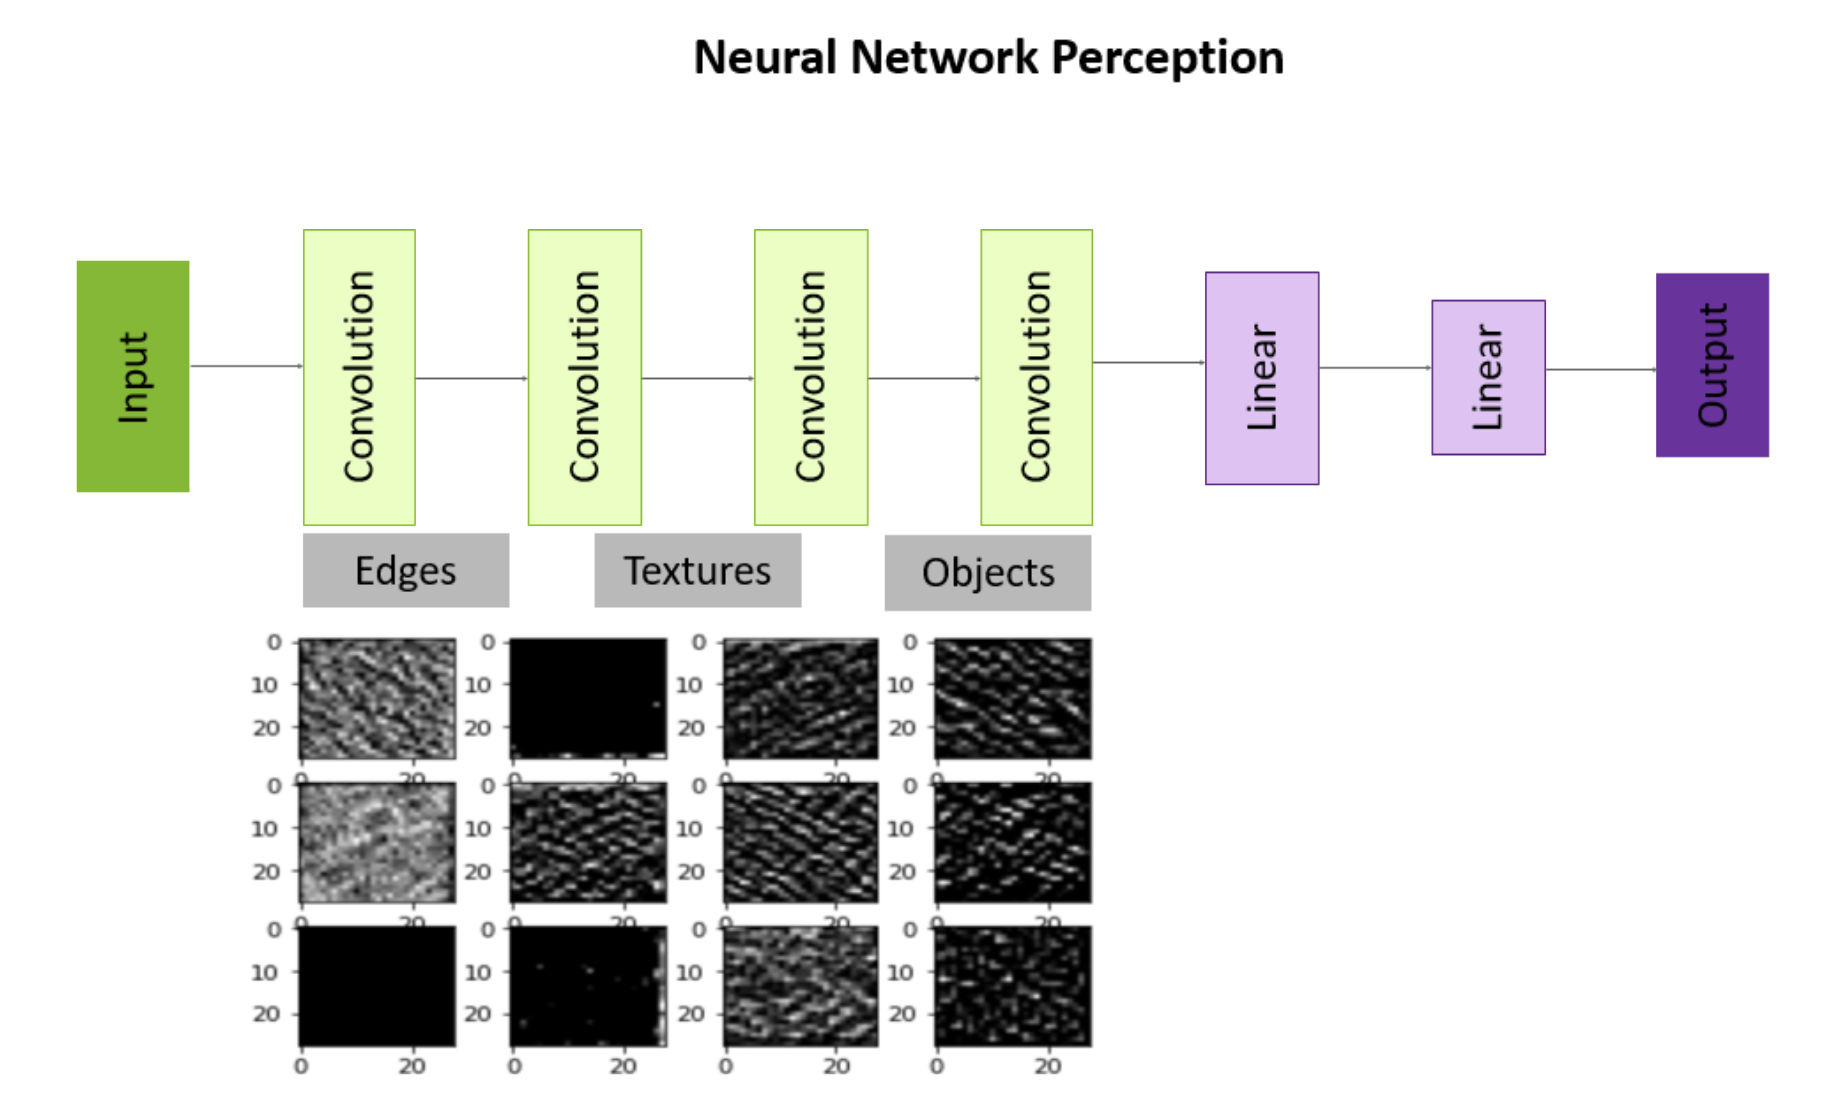
\includegraphics[width=0.9\textwidth]{../images/nnp_arch.png}

Max pooling is when you take the window to identify the maximum to represent the entire window when reducing the dimensions of an image. 

Dropout training refers to when you shutoff neurons during the training process to eliminate the possibility of one neuron overcontributing to the neural network. 

Batch normalization: scales weights / values of hidden layers to improve training. 
\subsection{\href{http://dli-e5d62e622240-a8611b.westus3.cloudapp.azure.com/lab/lab/tree/03_asl_cnn.ipynb}{Lab 3: Convolutional networks to avoid overfitting}}
\begin{enumerate}
    \item From the previous representation of our input data, we saw tensors that were flattened to represent data in a $1$-dimensional array. However, for the first convolutional layer of our model, we want to retain spacial information about which pixels are next to each other. We reshape our pixel representations such that it mimics some picturee representation. 
    \item This differs from the previous when we define our \verb|DATASET| class because we include a reshaping of the input data representation.
    \item Dataloader is created so that we set the batch size and shuffle for the training data so that the subset of the input data is randomized.
\end{enumerate}
Training accuracy was still higher than the validation accuracy. But sometimes it's not the model that needs work, it's the data. Require better examples. 

\section{\href{http://dli-e5d62e622240-a8611b.westus3.cloudapp.azure.com/lab/lab/tree/04a_asl_augmentation.ipynb}{Lab 4: Data Augmentation}}
Data Augmentation: changing the color hue, rotation, and flipping images to increasing our sample space. (Homography)
There are various random augmentation functions that we can deploy: 
\begin{itemize}
    \item \verb|RandomResizeCrop((IMG_WIDTH, IMG_HEIGHT), scale=(min, max), ratio=(1, 1))|\\
        \textit{ratio being aspect ratio}
    \item \verb|RandomHorizontalFlip()|
    \item \verb|RandomRotation()|
    \item \verb|ColorJitter(brightness, contrast, saturation, hue)|
\end{itemize}
Remembering that we can use the \verb|Compose()| function to group transform functions together, we can implement these data augmentation techniques as such: 
\begin{verbatim}
random_transforms = transforms.Compose([
    transforms.RandomRotation(5),
    transforms.RandomResizedCrop((IMG_WIDTH, IMG_HEIGHT), scale=(.9, 1), ratio=(1, 1)),
    transforms.RandomHorizontalFlip(),
    transforms.ColorJitter(brightness=.2, contrast=.5)
])
\end{verbatim}
So before we implement our training function we need to change the input to the model we built using this transformation process: \verb|output = model(random_transforms(x))| 

\subsection{Deploying the model:}
Because we have trained our model on a specific set of requirements, more spcifically, grayscale and $28 \times 28$ images, we need to ensure that any new images that we pass through comply with these requirements of our model- otherwise, the outputs mean nothing much. Here is an example of ensuring that images read into the model are grayscale: 
\begin{verbatim}
IMG_WIDTH = 28
IMG_HEIGHT = 28

preprocess_trans = transforms.Compose([
    transforms.ToDtype(torch.float32, scale=True), # Converts [0, 255] to [0, 1]
    transforms.Resize((IMG_WIDTH, IMG_HEIGHT)),
    transforms.Grayscale()  # From Color to Gray
])
\end{verbatim} After checking that our image is correctly reformated, we can start making predictions!
\begin{enumerate}
    \item Ensure that our reformatted image is \verb|.unsqueeze(index)| to add a dimension of 1 to the index of our "list / vector" representation of the image. 
\end{enumerate}
Once we ensure that our dimensions match up, we can push it through the \verb|model(batched_image)|. Batched image refers to how our model expects a batched input so placing our one image into a batch by itself allows us to generate a prediction for it alone. 

Once we do this, we recieve a prediction that is not like our labels but instead like this: \begin{verbatim}
tensor([[-25.0550,  12.9947,  -9.9380, -14.2813,  -3.0655,  -1.5400,  -1.0154,
        -14.3424,  -8.6212, -27.2385, -16.8412, -19.3476, -17.7453, -25.7918,
        -10.6322, -22.6966, -20.0060, -22.4649, -13.0284, -11.5978, -30.6815,
        -11.5446,  -5.6419, -28.9596]], device='cuda:0',
    grad_fn=<AddmmBackward0>)
\end{verbatim}
We see that this prediction output corresponds to a 24-length array that represents each letter of ASL that our input data might represent. So the \verb|argmax()| can help us identify which letter the input most likely represents. 

\section{Pre-trained Models: Very Deep Convolutional Networks for Large-scale image recognition}
\href{http://dli-e5d62e622240-a8611b.westus3.cloudapp.azure.com/lab/lab/tree/05a_doggy_door.ipynb}{Lab 5a} and \href{http://dli-e5d62e622240-a8611b.westus3.cloudapp.azure.com/lab/lab/tree/05b_presidential_doggy_door.ipynb}{Lab 5b}\\
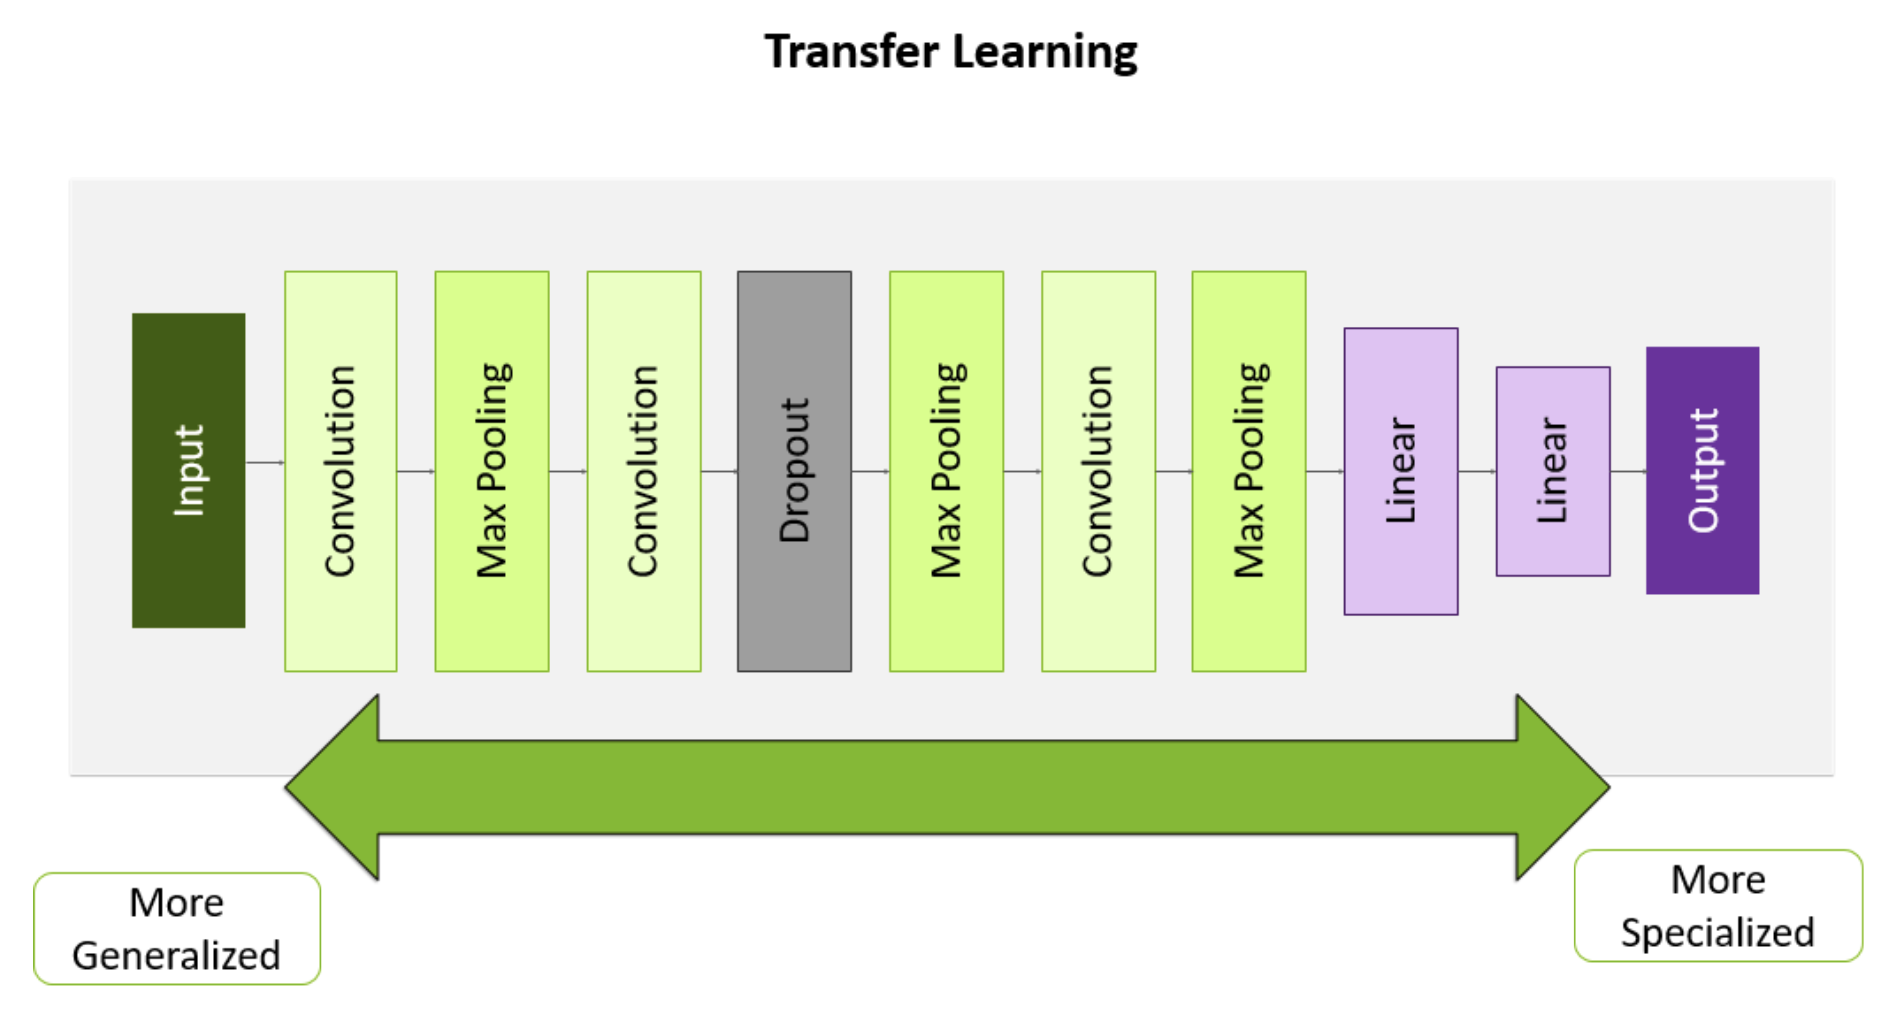
\includegraphics[width=0.9\textwidth]{../images/transferLearnign.png}\\
Freezing the model to avoid overfitting on the much smaller dataset. Data bias: when a subset of data that is over-represented in the dataset. 

Dreaming: feeding an image through layers of a network and utilizing gradient ascent instead of gradient descent. It exaggerates the features it detects! 

Using a pre-trained model, we want to ensure that we understand the pre-trained weights in order to match our $n$-dimensional representations and to freeze the base model when training our additional layers. Fine-tuning occurs after the initial training of the new layers and we can then unfreeze the base model to fine-tune by small learning increments. 

\section{Advanced Architectures}
\begin{itemize}
    \item Computer Vision: better our understanding of human perception of visual objects (color - RGB)
    \item NLP: generating human language but need to represent language numerically. How do we capture sentence structure and semantic subtleties? 
\end{itemize}

\section{Natural Language Processing}
From our dictionary of words, we assign each input word / token to a neuron like utilizing One-hot encoding. 
Embedding handles our large dictionary size such as going from a layer with a higher number of neurons to a lower number of neurons. Suppose that some embedding outputs 3 encodings per input. When we take two embedding matrices and multiply them together, we can derive an attention matrix. 

BERT, Bidirectional Encoder Representations for Transformers by Google was trained towards predicting a missing word from a sequence and predicting a new sentence after a sequence of sentences. 

Autoencoders are used to represent an input with a lower dimensional medium in order to reconstruct the same output. An encoder allows us to storage large amounts of data with low dimensional representation. This can be applied to the detection of anomalies and security purposes. 
\begin{itemize}
    \item Variational Autoeconder: generative AI for images
    \item Diffusion Models: Taking a noisy image and slowly remove small amounts of noise until we generate a somewhat noise free image (Stable Diffusion!)
    \item Reinforcement Learning; Put off a reward for now in hopes of attaining a greater reward later. Applications in Robotics and Finance
\end{itemize}
\end{document}